\cleardoublepage
\newpage
\ifdefined\EnableIncludeImages
    \ThisULCornerWallPaper{1.0}{chapterimage.eps}
\fi
\chapter{Zandor}

Após a morte de Zorra, toda a família ficou muito triste, pois apesar de seus maus costumes, ela sempre foi muito amorosa conosco, por isso sentíamos sua falta como se fosse um membro da família. 
Assim, passamos muito tempo chorando, sobretudo minhas irmãs e eu, que ainda éramos crianças. 
Muitas vezes vi a Teodosia ---  minha irmã mais velha, a qual carinhosamente chamávamos ``Tulaco'' ---, iniciar a chorar em silêncio ao ver o lugar onde Zorra dormia; inclusive Diofelia  --- ``Dio'', a minha irmã mais nova ---, apesar de sua curta idade, já sabia distinguir a morte e a ausência que esta deixa. 
Eu também chorava, talvez mais do que elas, porque Zorra era minha companheira fiel, ela me seguia a todos os lugares onde eu ia; pois, ao ser o filho homem da casa, eu era quem tinha que sair a trabalhar na chacra com meu pai, e Zorra sempre fazia mais alegres e memoráveis esses momentos.
Nosso único conforto era que tínhamos a Zandor; nós amávamos ele por ser o último presente que Zorra nos deixou.
Eu olhava para Zandor, todo pequeno e pretinho e achava ele muito lindo; sua presença me dizia que de alguma forma, uma parte de Zorra ainda estava conosco. 
Assim, Zandor cresceu sendo criado com muito cuidado e carinho por todos nós;
entretanto a pessoalidade de Zandor era distinta da pessoalidade de sua mãe, ele era um cachorro muito honrado e era evidente para nós que não tinha nenhuma dos maus costumes de Zorra. 
\ifdefined\EnableIncludeImages
\begin{wrapfigure}{r}{0.45\textwidth}
  \begin{center}
  \vspace{-20pt}
    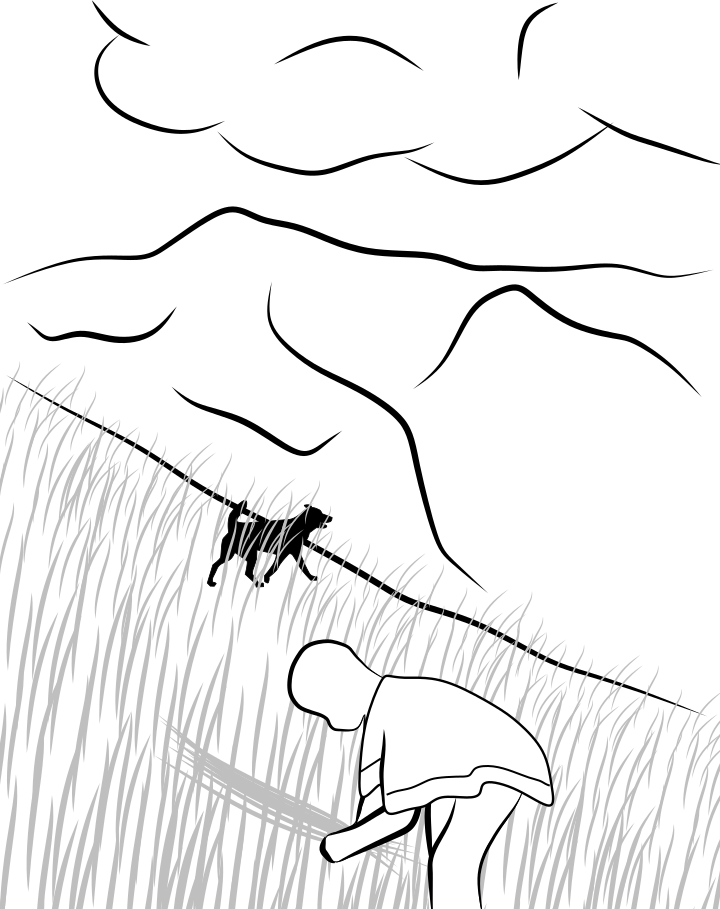
\includegraphics[width=0.43\textwidth]{pasto-zandor-aulicha}
  \end{center}
  \vspace{-20pt}
  %\caption{Figo das índias.}
\end{wrapfigure}
\fi
Desde pequeno eu levei Zandor a todas as minhas caminhadas pela serra; como minha família tinha vacas, eu tinha que ir dar-lhes comida e atendê-las, e comumente recompensava a Zandor por sua companhia dando-lhe leite fresco, que eu mesmo ordenhava para matar a nossa sede. 
Com todos esses cuidados, em pouco tempo Zandor virou um cachorrinho forte e muito brincalhão,
ele me ajudava a cuidar as vacas e assustava os pássaros que vinham comer as sementes na chacra; quando eu gritava seu nome, ele vinha correndo e se parava frente a mim com a marcialidade de um soldado diante do seu general; ele era tão inteligente quanto uma pessoa e bem mais obediente que eu mesmo.

Um dia, quando estava no campo com Zandor, observamos que uma perdiz saía voando desde uns arbustos; para Zandor, que ainda era filhote, essa foi a primeira vez que ele viu uma perdiz; eu, pelo contrário, já tinha experiência com essas aves e sabia que próximo a esse lugar acharíamos um ninho, ovos ou crias. 
Automaticamente gritei: 
--- Zandor! Vamos buscar ovos! --- 
Ele latiu ao sentir minha empolgação e avançou junto a mim na direção que eu indiquei para ele. 
Era gostoso ver Zandor, pequeno, porém corajoso, batendo seu rabinho, cheirando para todos os lados, levantando e recolhendo suas orelhas; como se, nessa sua primeira missão de busca, quisesse demonstrar sua eficácia usando ao máximo todos seus sentidos. 
Só procuramos uns minutos e de repente os vimos --- olha Zandor! Ovos! --- gritei, ele latiu como afirmando minha exclamação, e me acerquei ao ninho para recolher todos os ovos; Zandor não pegou nenhum, ele só me olhava contente enquanto eu os colocava num saquinho de tecido para protegê-los e levá-los a casa. 


Este procedimento se tornou comum, e cada vez que eu saía a procurar as vacas, também aproveitava para procurar ovos de perdiz com Zandor; quando os achávamos, eu os levava muito contente a minha mãe; de modo que, todos os dias nós voltávamos com 8, 12 ou até 15 ovos. 
Com o passar dos meses Zandor virou um especialista em encontrar ovos, além de que ele já não era um filhote, e eu não precisava acompanhá-lo; assim, enquanto eu trabalhava, ele saía por conta própria a procurar ovos; no instante que ele os achava, latia para mim, repetidas vezes e sem descanso, até chamar minha atenção, de modo que minha única missão era recolhê-los e levá-los para casa.
\ifdefined\EnableIncludeImages
\begin{wrapfigure}{r}{0.45\textwidth}
  \begin{center}
  \vspace{-20pt}
    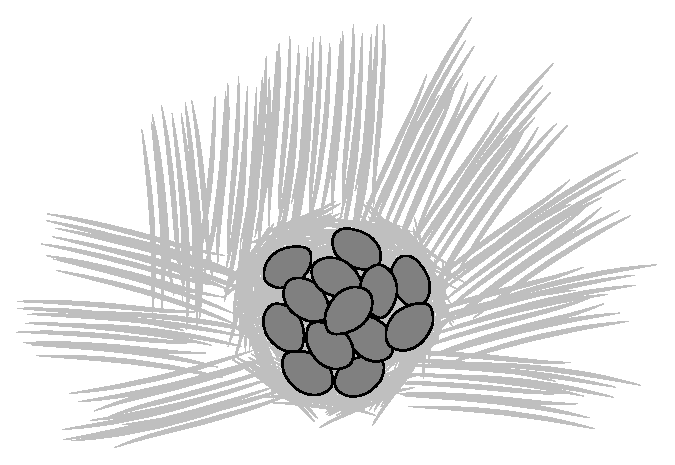
\includegraphics[width=0.43\textwidth]{huevos.eps}
  \end{center}
  \vspace{-20pt}
  %\caption{Figo das índias.}
\end{wrapfigure}
\fi
Algumas vezes cozinhávamos os ovos, outras vezes os fritávamos; sendo que numa dessas ocasiões, meu pai chegou em casa enquanto estávamos cozinhando-os,--- e esses ovos?--- perguntou ele, 
e nós contentos e cheios de orgulho respondemos: 
--- Zandor achou!---
Ele meditou um pouco e replicou: 
--- Zandor achou... e que coisa deram a ele? --- 
A pergunta nos pegou de surpresa e falamos em voz baixa: 
--- Nada pai, só a comida da casa... --- meu pai nos olhou e indicou calmamente: 
--- Se ele foi quem achou, ele também deve participar ---; 
nesse momento meu pai pegou um ovo cru e deu para o cachorro, Zandor pegou contente o ovo e lambeu ele até sobrar só a casca; a partir de então Zandor se acostumou a comê-los sempre que lhe ofereciam. Assim, cada vez que ele encontrava ovos, eu os levava a casa, os entregava a minha mãe e ela na sua vez entregava dois a Zandor; porém nunca lhe dávamos os ovos quando ele os encontrava, somente na casa, ele por sua parte sabia esperar e nunca pegou nenhum, só esperava pacientemente o momento que minha mãe entregasse a ele seus ovos e ia contente a seu cantinho a comê-los.


Para mim Zandor era maravilhoso, a qualquer lugar que ia ele me acompanhava, quando estava triste ele se sentava a meu lado e até chorava comigo fazendo um sonido agudo, que eu sentia cheio de solidariedade. 
Por outro lado, se ele percebia que eu estava contente, levantava suas orelhinhas e iniciava a pular e correr de um lado a outro; assim, durante muito tempo, andamos e crescemos juntos... o tempo passou, e eu cumpri oito e logo nove anos.

Um dia meu pai decidiu abater um boi; lá na serra não se mata um boi sem nenhum motivo, só em ocasiões importantes como festas regionais, casamentos ou eventos semelhantes; sem embargo, eu sabia que nessa época não tínhamos nenhuma festividade e pensava que a meu pai simplesmente ocorreu-lhe abater o boi sem nenhum motivo, mas não era assim. 
Eu tinha um irmão mais velho que morava na capital, em Lima; eu não o conhecia, só sabia de sua existência, pois meus pais sempre falavam sobre sua vida lá e se referiam a ele como ``Seve'', pelo que nessa época eu pensava que ele se chamava dessa forma, não obstante, seu nome não era esse e sim Severino; eu não o conhecia porque viajou a Lima quando eu era muito pequeno, seguramente o vi quando era um bebê, mas eu não tinha lembrança disso. 
Assim, meu pai e minha mãe tinham a intenção de fazer charque para mandar-lho a meu irmão como presente, pelo que com esse fim decidiram abater o boi e prepararam cuidadosamente sua carne com muito sal.

\ifdefined\EnableIncludeImages
\begin{wrapfigure}{r}{0.49\textwidth}
  \begin{center}
  \vspace{-20pt}
    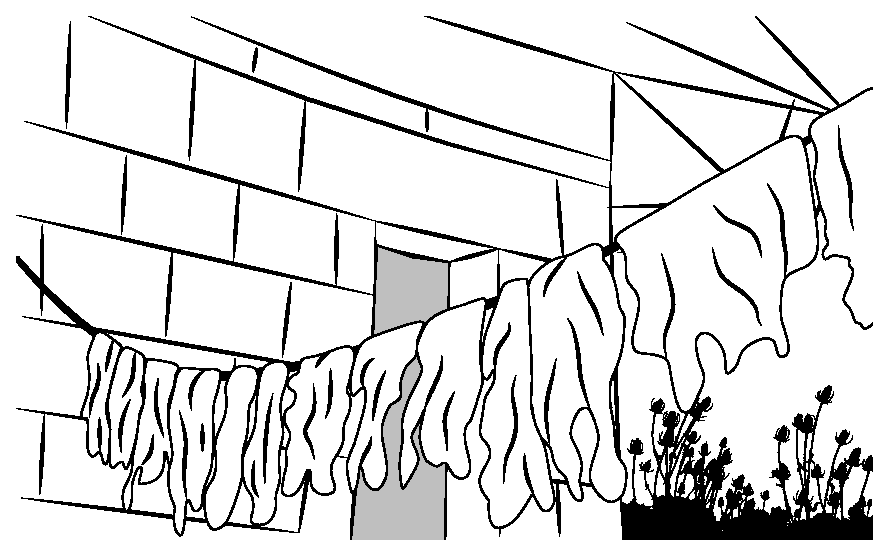
\includegraphics[width=0.47\textwidth]{charque.eps}
  \end{center}
  \vspace{-20pt}
  %\caption{Zandor}
\end{wrapfigure}
\fi
Nosso lar estava composto por uma casa pequena e uma grande, ambas separadas vários metros entre si; nossa família morava na casa grande e usávamos a pequena para guardar ferramentas, grãos e, em geral, alimentos não perecíveis. Perto da casa pequena tínhamos duas figueiras; esse dia meu pai usou uma delas para amarrar uma corda até a casa pequena, e sobre ela pendurou a carne para secar-lha com o sol, porém ele decidiu pendurar uma perna de boi no tronco da outra figueira, pois essa peça de carne pesava muito.
Lá o costume é recolher a carne e levá-la para a casa durante a noite, para que os animais de hábitos noturnos não venham a comê-la, de modo que no dia seguinte, pela manhã, com os primeiros raios do sol, a carne era novamente pendurada; não obstante, esse dia meu pai recolheu só o charque que estava pendurado na corda e esqueceu a perna que tinha colocado na outra figueira. 
O pior foi que ali, onde meu pai deixou a carne, tranquilamente qualquer cachorro, zorro, ou outro animal carnívoro da serra, poderia pegá-la facilmente, sem a necessidade de pular, uma vez que não estava a muita altura.

Essa noite Zandor não parou de latir; nós desde a casa grande só escutávamos seu barulho com curiosidade, dado que nenhum membro da família lembrou da perna pendurada na figueira; pelo barulho só reconhecíamos que algumas vezes chegavam outros cachorros, outras vezes não escutávamos nenhum outro animal, só o Zandor latindo com muita raiva e força; meu pai, bravo pelo ruído, só falava: 
--- Que coisa quer esse cachorro que não nos deixa dormir! --- Porém ele não saía da casa grande a indagar sobre a situação; eu tinha muito medo por tudo o que estava acontecendo; pois, lá na serra, se contam histórias dos seres que habitam a noite. 
Alguns dizem que de noite anda o ``cuco''\footnote{Também chamado, coca ou coco, este é um ser mítico, uma espécie de fantasma, bruxa ou bicho-papão que anda de noite pelos caminhos.}, e as crianças tínhamos um terror extremo a esse ser; para piorar a situação meu pai tinha o costume de contar-nos histórias de suas viagens, de como de noite achou o cuco nos caminhos da serra, ou também que em algum povoado perto o cuco tinha matado algum vizinho, que tinha chupado o sangue de outro ou simplesmente assustado a algum caminhante noturno; devo reconhecer que apesar do terror que me causavam as histórias do meu pai, eu gostava de conhecê-las e passar medo ouvindo-as; ele sempre me contava suas aventuras de quando saía a trabalhar a outras cidades e das coisas que viu, dos problemas que aconteciam no caminho e dos personagens que apareciam quando ele se deslocava a pé.

\ifdefined\EnableIncludeImages
\begin{wrapfigure}{r}{0.49\textwidth}
  \begin{center}
  \vspace{-20pt}
    \includegraphics[width=0.47\textwidth]{AgriornisSolitariaSmit.jpg}
  \end{center}
  \vspace{-20pt}
  %\caption{Zandor}
\end{wrapfigure}
\fi
Por exemplo, um dia meu pai me contou que quando estava viajando desde nosso povo até ``Cangallo'', um povoado vizinho, no meio do caminho a noite o atrapou, e ele iniciou a procurar entre os trilhos alguma casa que pudesse darlhe pousada; enquanto ele estava nessa tarefa, escutou um pássaro ao qual nós na serra chamamos ``huaychao''\footnote{Também escrito como waychaw, esta é uma palavra quéchua que significa: avisar, anunciar, advertir ou notificar. ``Huaychao'' é uma onomatopeia do som que faz a ave cujo nome científico é Agriornis montanus.}, cujo canto é de mau augúrio.
Meu pai falava que quando o ``Huaychao'' canta é porque o mal está perto, que ele canta porque viu o mal andando, talvez na forma de algum ``jarjacha''\footnote{Também chamado carcaq ou qarqacha.}. Para nós os jarjachas são seres da noite, são pessoas que se levantam dos seus túmulos, pois ao ter feito coisas terríveis em vida estão condenados a não morrer e vagar de noite entre o sofrimento e a ira. 
Então, meu pai sempre me advertia muito sério, que se na noite escutava ao huaychao, devia ter muito cuidado porque seguramente um jarjacha estava perto. 
Na sequência dos fatos, quando meu pai escutou ao huaychao, iniciou a correr pulando pedras e atravessando riachos até que, só e assustado, achou uma casa; rapidamente tocou a porta e desde dentro escutou uma voz de mulher que lhe perguntava: 
--- Boa noite! Quem anda ali? ---
Meu pai todo assustado tentou lhe explicar que era só um viajante, que a noite tinha chegado em médio do seu caminho e que precisava só um lugar para dormir; a senhora desde o interior lhe respondeu que, da mesma forma que ele falou, seres que não são pessoas, cucos, andam pela noite enganando aos moradores para conseguir entrar a suas casas, 
--- de repente você é um deles! --- indicou a senhora e negou a meu pai um lugar para dormir; ele insistiu com a voz tremida pelo medo, porque sabia que tudo isso era verdade, pois ele já tinha escutado ao huaychao e sabia que o mal estava perto; por fim, após muito insistir, a senhora se comoveu e deixou entrar a meu pai à casa. 
A senhora, toda curiosa pela situação, perguntou a meu pai por quê andava de noite, e ele explicou que só estava tentando ir de Occo a Cangalho, porém teve problemas no caminho e a noite lhe ganhou; imediatamente a senhora respondeu em tom maternal: 
--- Por quê você anda de noite? Só ontem um jarjacha comeu uma pessoa, agora esse vizinho está morto, hoje mesmo enterramos ele ---.
Por todas essas histórias, sair da casa grande de noite, só porque o cachorro latia, era uma completa temeridade; até meu pai tinha medo de sair, ele só gritava para Zandor desde dentro da casa, segurando sua ``guaraca''\footnote{Corda muito versátil que pode ser usada como cinto de calças ou para disciplinar crianças desobedientes.}, golpeando com ela a parede. 
Os demais membros da família só escutávamos resignados, intentando dormir apesar do barulho.

Assim, a noite passou, e praticamente nenhum de nós conseguiu dormir; quando os primeiros raios do sol tocaram a nossa janela, todos nós saímos em direção da casa pequena e para nossa surpresa vimos a perna de boi pendurada na figueira, para nós foi evidente que de noite os animais do campo tinham chegado a comer a carne e Zandor tinha defendido ela, brigando, latindo e sem dormir.
\ifdefined\EnableIncludeImages 
\begin{wrapfigure}{r}{0.47\textwidth}
  \begin{center}
  \vspace{-0.5cm}
    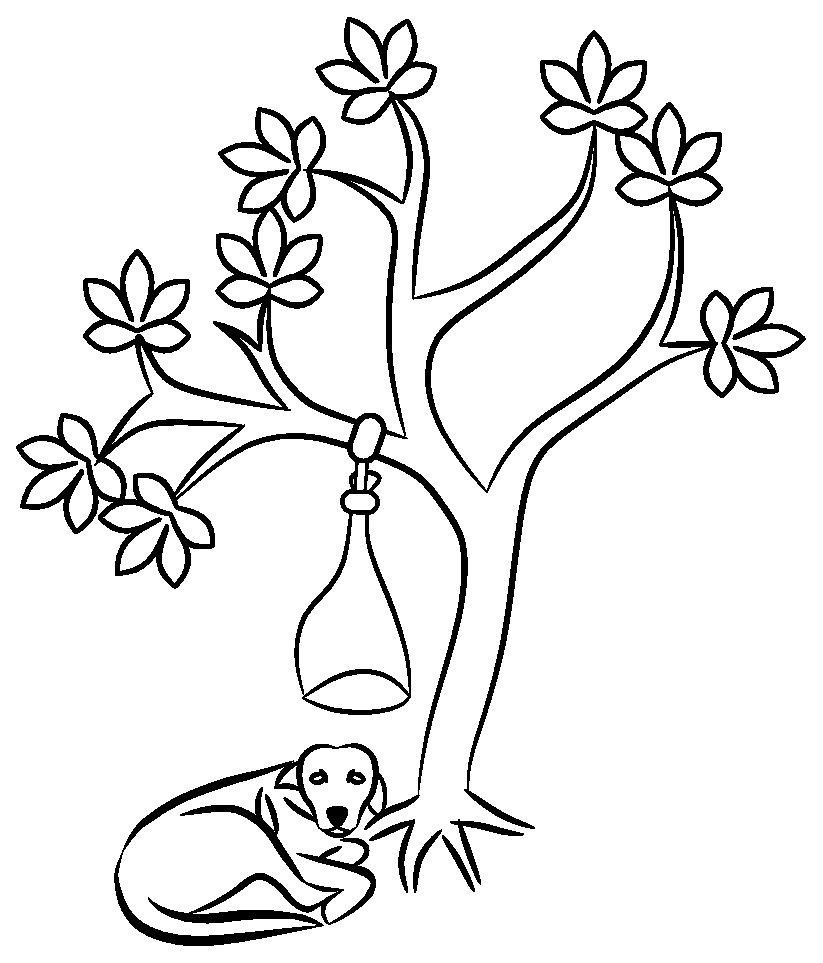
\includegraphics[width=0.45\textwidth]{perro-fiel-1.eps}
  \end{center}
  \vspace{-0.5cm}
  %\caption{Zandor}
\end{wrapfigure}
\fi
Ele estava aconchegado encolhido em forma de bolinha abaixo da perna de boi e ao nos ver chegar só nos dirigiu um olhar cansado enquanto abanava o rabinho; meu pai se admirou pelo desempenho de Zandor, pois a carne estava intacta. 
--- Como me olvidei da perna! Por isso chegavam os cachorros! --- exclamou meu pai, 
automaticamente entrou à casa, pegou uma faca, cortou com ela um pedaço grande de carne na perna de boi, ainda pendurada na figueira, e a entregou a Zandor como um prêmio; só nesse momento ele olhou a carne com vontade, pegou seu prêmio e foi para o canto dele para comer.

Assim, Zandor cresceu sendo sempre um cachorro honrado, se você não dava alguma coisa, ele não pegava, por isso toda a família o respeitava. Além disso, no campo, os cachorros sempre são bem cuidados; eles comem a mesma comida dos donos de casa e são tratados com carinho, sendo eles considerados como membros da família.

